\documentclass[11pt]{article} % use larger type; default would be 10pt

\usepackage[utf8]{inputenc} % set input encoding (not needed with XeLaTeX)

\usepackage{tikz}
\usetikzlibrary{decorations.pathmorphing}
\begin{document}


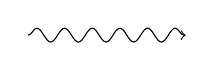
\begin{tikzpicture}
\draw [->,decorate,decoration=snake] (0,0) -- (2,0);
\end{tikzpicture}

\begin{tikzpicture}
\path[use as bounding box] (0,0) rectangle (0,2);
\draw [->,decorate,
decoration={snake,amplitude=.4mm,segment length=2mm,post length=1mm}]
(0,0) -- (3,0);
\end{tikzpicture}

% WITH MULTI-LINE TEXT:  OPTION 1
% specify an align=center and then use the \\ command
% to enforce the line breaks at the desired positions.
\begin{tikzpicture}
	\path[use as bounding box] (0,0) rectangle (0,3);
	\draw [->,decorate,
			decoration={snake,amplitude=.4mm,segment length=2mm,post length=1mm}]
				(0,0) -- (3,0)
				node [above,align=center,midway]
{replacement of\\ the \textcolor{red}{capacity}\\ by \textcolor{red}{two places} };
\end{tikzpicture}

% WITH MULTI-LINE TEXT: OPTION 2
% Instead of "specifying the line breaks by hand," you can also specify a width 
% for the text and letTEX perform the line breaking for you:
\begin{tikzpicture}
	\path[use as bounding box] (0,0) rectangle (0,3);
	\draw [->,decorate,
		decoration={snake,amplitude=.4mm,segment length=2mm,post length=1mm}]
			(0,0) -- (3,0)
		node [above,text width=3cm,align=center,midway]
	{replacement of the \textcolor{red}{capacity} by\textcolor{red}{two places} };
\end{tikzpicture}

\end{document}